\chapter{Methodology}
\label{chap:methodology}

\section{Point Cloud Data}
\label{sec:point_cloud_data}

This project aims to work with large amounts of point cloud data. It contains arrays of three-dimensional coordinates and the four-component color data. The color information does not affect performance strongly. However, the massive number of points itself introduces the heavy load on computer resources. For improving the performance of visualization software, this work proposes two methods: Generating Levels of Detail (LODs) and Creating a heightmap.


\section{Data Preprocessing}
\label{sec:data_preprocessing}

The data itself is stored in a PCAP file as captured packet stream from the lidar. It is necessary to preprocess original files before working on the point cloud. The preprocessing involves three main steps: converting the file from PCAP format to the LAS format, importing the LAS file into Unity, and splitting the point cloud data into chunks.

\subsection{Converting to LAS format}
\label{subsec:converting_to_las}

PCAP is an open network traffic capturing system that uses its own \texttt{.pcap} file format [citation here]. As mentioned above, the file contains the recorded packet stream from the lidar at the time of capturing the area. It means that the data is stored as individual captures from various perspectives and at different times.
This step collects the data stream into the single point cloud, which represents the whole captured area. The resulting point cloud is stored in LAS format [citation here].
The VeloView is a software for previewing the data from lidars and converting it to different formats [citation here]. It is used to preview the PCAP stream and convert it to the LAS format for further processing.

\subsection{Importing LAS files into Unity}
\label{subsec:importing_las_unity}

As this project uses the Unity engine as a base, it is essential to have the ability to read LAS files within its programming environment. Importing the LAS file into Unity is being done with the help of the LASzip.NET library.
LASzip is a library for compressing, decompressing, and parsing the lidar data from LAS files [citation here]. LASzip.NET is a wrapper for LASzip which makes it possible to utilize the functionality of the main library within the .NET environment which in turn is being used for programming in the Unity engine.

\subsection{Splitting into chunks}
\label{subsec:splitting_into_chunks}

For the proposed methods it is crucial to split the point cloud into smaller units (chunks) that are easier to process. It also helps to process the data in a parallel manner, thereby making the algorithms more scalable in terms of performance.

In terms of the given project, the chunk is a space bounded by computed borders. It has a position, and a size, which is the same for its width, height, and depth. 

\paragraph{Algorithm}
At the start, the algorithm computes the number of chunks in three dimensions using the formula \ref{formula:n_chunks}. It uses the predefined chunk size and the boundaries of the point cloud object.

The number of chunks for an axis $\alpha$ is computed as follows:

\begin{equation}
\label{formula:n_chunks}
N_{chunks}^\alpha = \lceil BBox_{max}^\alpha - BBox_{min}^\alpha \rceil / Size_{chunk}
\end{equation}

For that, the chunk grid will have the size of $N_{chunks}^X \times N_{chunks}^Y \times N_{chunks}^Z$.

The chunks are stored in a three-dimensional array. It means that each chunk has its corresponding index.

After that, the algorithm iterates overall points and computes the exact chunk index they correspond to, based on their global position.

The chunk index for a point with position $pos$ on an axis $\alpha$ is computed as shown on formula \ref{formula:point_index}:

\begin{equation}
\label{formula:point_index}
Index_{pos}^\alpha = \left \lfloor \frac{pos^{\alpha} - BBox_{min}^\alpha}{Size_{chunk}} \right \rfloor
\end{equation}

In the end, the points are stored within chunks. It is now possible to read the point cloud data in chunks.


\section{Method 1: Generating LODs}
\label{sec:generating_lods}

The level of detail defines the complexity of the model [citation here]. For this project, the level of detail adjusts the number of points shown for a particular object.

The LOD of L shows L\% of all points of an object. For example, a chunk with LOD 100 renders all its points while LOD 70 renders 70\% of chunk points. The algorithm does this by introducing the render probability.

\begin{equation}
\label{formula:render_probability}
P_{Render} = \frac{LOD}{100}
\end{equation}

The first approach is to generate different levels of detail for each chunk so it will be possible to show fewer points for chunks that are far enough not to notice the low-detailed chunk.

\newpage

\section{Method 2: Creating a Mesh}
\label{sec:creating_mesh}

Mesh is a data structure that contains vertices, texture data, normals, and other details [citation here]. Later, the engine  combines the mesh data and draws it on the scene.

Mesh creation consists of several stages:

\begin{enumerate}
    \item Map the point cloud into grid.
    \item Generate triangles.
    \item Fill the mesh.
\end{enumerate}


\subsection{Vertex grid}
\label{subsec:vertex_grid}

Meshes consist of vertices. We first create a set of vertices that later will form the mesh.

First, the algorithm generates a flat grid of vertices. It is a square-bounded grid-aligned region that has a specified side length. It has $length \times length$ dimensions. Each point at this plane has a height value initially set to zero.

\begin{figure}[ht]
    \centering
    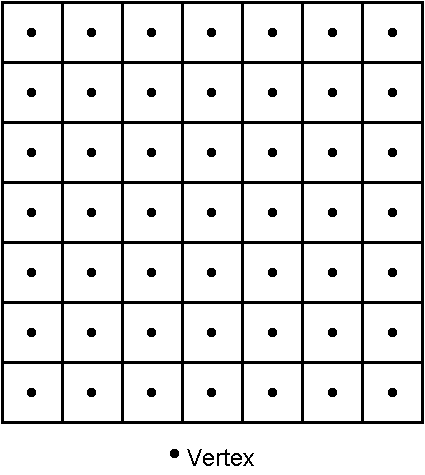
\includegraphics[width=0.3\textwidth]{methodology/vertex-grid.pdf}
    \caption{Vertex grid}
    \label{fig:vertex_grid}
\end{figure}


\subsection{Mapping the point cloud into grid}
\label{subsec:map_to_grid}

\subsubsection{Occurrence map}

To determine where the mesh triangles should appear, the algorithm fills the occurrence map. The \textbf{occurrence map} tracks the appearance of points within the specified grid cells. It has the same size as the vertex grid. All map values are initially set to false. It means that no points have been noticed here yet.

The algorithm maps each point within a chunk to a specific occurrence map cell.

\begin{figure}[ht]
    \centering
    
    \begin{subfigure}[t]{0.3\textwidth}
        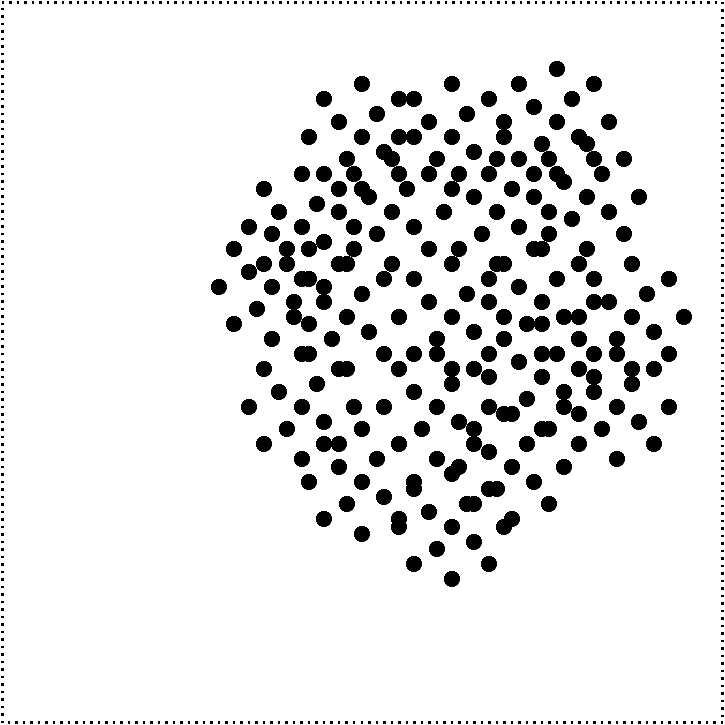
\includegraphics[width=\textwidth]{methodology/point-cloud-plot.pdf}
        \caption{Example of point cloud data in two dimensions.}
    \end{subfigure}
    % side-to-side
    \begin{subfigure}[t]{0.3\textwidth}
        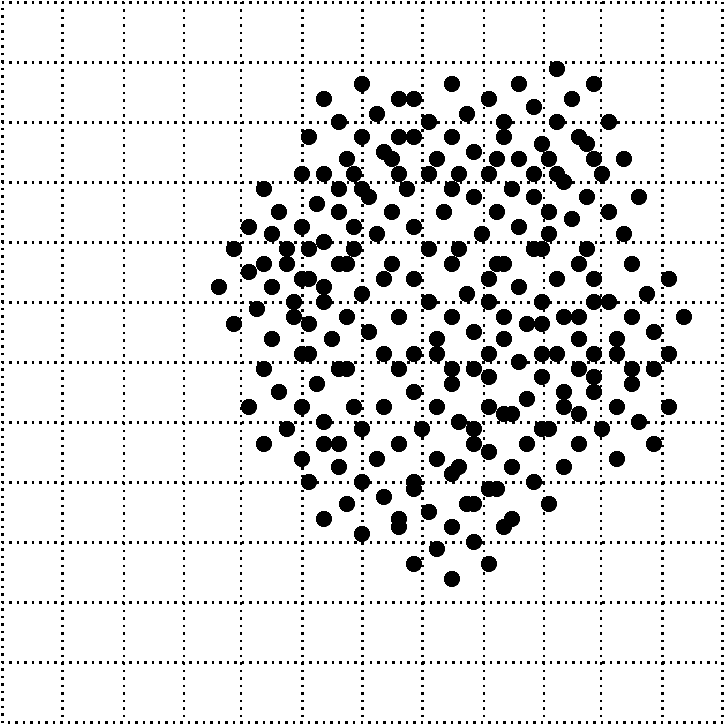
\includegraphics[width=\textwidth]{methodology/occurrence-grid.pdf}
        \caption{Occurrence grid.}
    \end{subfigure}
    
    \begin{subfigure}[t]{0.4\textwidth}
        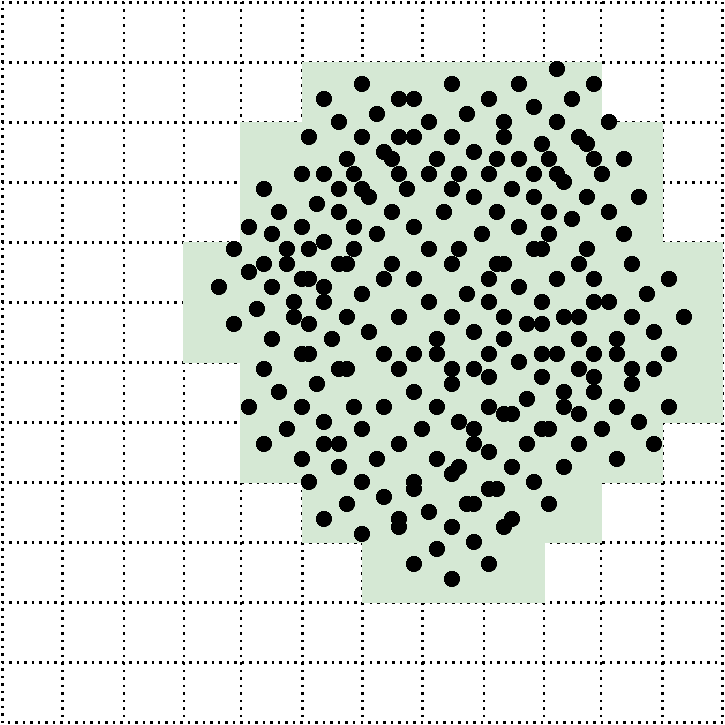
\includegraphics[width=\textwidth]{methodology/occurrence-map-applied.pdf}
        \caption{Applied occurrence map.}
    \end{subfigure}
    
    \caption{Applying occurrence map.}
    \label{fig:occurrence_map}
\end{figure}

The occurrence map represents a strictly aligned version of the point cloud viewed from above.


\subsubsection{Calculating cell indices}

To work with grid, the algorithm should calculate a cell index for each point.

To calculate an index, it should do the following:
\begin{enumerate}
    \item Calculate the local coordinate within chunk.
    \item Divide the local coordinate by cell size.
    \item Truncate the result down.
\end{enumerate}

See the formula \ref{formula:cell_coordinate}.

\begin{equation}
\label{formula:cell_coordinate}
Cell coordinate(p) = \left \lfloor \frac{Pos(p) - chunk origin}{cell size} \right \rfloor
\end{equation}


\subsection{Traversing points and emitting new vertices}
\label{subsec:emitting_vertices}

After initializing the vertex grid and occurrence map, the algorithm starts processing the point cloud itself.

For each point in a point cloud, the algorithm  calculates its grid cell index and fills the corresponding cell in the vertex grid and occurrence map.

At the vertex grid, the algorithm compares the height value stored in the cell and the height of the point (its Y coordinate). If the value stored in the grid is less than the point height, the algorithm writes the point height to the grid cell.

At the occurrence map, the algorithm tracks the occurrence of the points in the grid cells. If a point belongs to the cell, that cell is marked as visited.


\begin{algorithm}
    \For{point \textup{p} in \textup{points}}{
        x, y, z $\gets CellCoords(p.Position)$\;
        
        \If{vertices[x,z].y < y}{
            vertices[x,z].y = y\;
        }
        
        occurrenceMap[x, z] $\gets$ \textbf{true}\;
    }
\end{algorithm}


\subsection{Generating triangles}
\label{subsec:generating_triangles}

After finishing building the vertex grid, it is necessary to combine vertices into triangles that are going to form the mesh. To achieve this, the algorithm uses the vertex grid and the occurrence map from the previous step.

The algorithm traverses the vertex grid. The main goal is to connect three adjacent points in the grid into a triangle.

The vertex grid is represented as a two-dimensional array. On each iteration, the algorithm checks each possible triangle appearance. If a triangle exists, its vertices are recorded.

To check whether it is possible to create a triangle, the algorithm checks two adjacent points on the occurrence map. At the point $(X, Y)$, it checks whether $\left \langle (X, Y), (X+1, Y) (X, Y+1) \right \rangle$ and $\left \langle (X+1, Y), (X, Y+1), (X+1, Y+1) \right \rangle$ appear on the occurrence map. If they do, the corresponding triangles are recorded.

\begin{algorithm}
    \For{\textup{x} in 1..\textup{width}}{
        \For{\textup{y} in 1..\textup{width}}{
            \If{occuranceMap[x, y] and occuranceMap[x+1, y] and occuranceMap[x, y+1]}{
                recordTriangle(x, y, x+1, y, x, y+1)\;
            }
            \If{occuranceMap[x+1, y] and occuranceMap[x, y+1] and occuranceMap[x+1, y+1]}{
                recordTriangle(x+1, y, x, y+1, x+1, y+1)\;
            }
        }
    }
\end{algorithm}

<Illustration here>
